% Diagram of Android activity life cycle
% Author: Pavel Seda 
\documentclass[border=10pt]{standalone}
\usepackage{tikz}
\usetikzlibrary{arrows.meta}

\begin{document}  

\begin{tikzpicture}[>=Latex,
						leftWidth/.style={minimum width=0.525cm},
            leftHeight/.style={minimum height=3cm},
						topWidth/.style={minimum width=3cm},
						topHeight/.style={minimum height=1.8cm},
						bottomWidth/.style={minimum width=3cm},
						bottomHeight/.style={minimum height=3.2cm},
						cylinderWidth/.style={minimum width=2.05cm},
						cylinderHeight/.style={minimum height=3.6cm}
            ]
  
  \node[inner sep=0pt] (ucase)
    {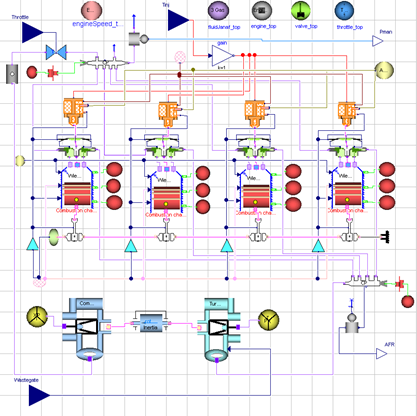
\includegraphics{use_case.png}};
		
	\node[anchor=west, leftHeight, leftWidth] (leftBar) at (ucase.west) {};

  \node[anchor=east,topHeight, topWidth, yshift=-0.9cm] (topBar) at (ucase.north east) {};
  \node[anchor=east,bottomHeight, bottomWidth, yshift=1.6cm] (bottomBar) at (ucase.south east) {};
	
	\node[anchor=south,draw=blue, densely dashed, cylinderHeight, cylinderWidth, xshift=-5.75cm, yshift=0.1cm] (cylinder1) at (bottomBar.north) {};	
	\node[anchor=west,draw=blue, densely dashed, cylinderHeight, minimum width=1.9cm, xshift=0.02cm] (cylinder2) at (cylinder1.east) {};
	\node[anchor=west,draw=blue, densely dashed, cylinderHeight, minimum width=1.9cm, xshift=0.02cm] (cylinder3) at (cylinder2.east) {};
	\node[anchor=west,draw=blue, densely dashed, cylinderHeight, minimum width=1.9cm, xshift=0.02cm] (cylinder4) at (cylinder3.east) {};
	
	\node[anchor=east,xshift=-1cm] (airpathlabel) at (leftBar.west) {Airpath};
	\node[anchor=west,xshift=1cm,yshift=2cm] (cylinderlabel) at (cylinder4.east) {Cylinders};
	
	\draw[->,red] (airpathlabel) -- (leftBar.west);
	\draw[->,red] (cylinderlabel.west) -- (cylinder4.east);
	\draw[->,red] (cylinderlabel.west) -- (cylinder3.east);
	\draw[->,red] (cylinderlabel.west) -- (cylinder2.east);
	\draw[->,red] (cylinderlabel.west) -- (cylinder1.east);
	

  \draw[blue, densely dashed] (topBar.north east) -- (topBar.north -| leftBar.west) -- (bottomBar.south -| leftBar.west) -- (bottomBar.south east) -- (bottomBar.north east) -- (bottomBar.north -| leftBar.east) -- (topBar.south -| leftBar.east) -- (topBar.south east) -- cycle;
	
	
 
  \end{tikzpicture}
\end{document}